\documentclass[11pt,letterpaper]{article}
\usepackage[T1]{fontenc}
\usepackage{mathptmx}
\usepackage[margin=1in]{geometry}
\usepackage{graphicx,array}
\newcommand{\toprule}{\hline}\newcommand{\midrule}{\hline}\newcommand{\bottomrule}{\hline}
\linespread{1.08}\selectfont
\title{Recurrent mutation patterns in antimicrobial-peptide evolution experiments: a preregistered, descriptive audit with an unmet discovery gate\\[2pt]\large mega27-09e (ResistPep), status report of 8 October 2026}
\author{Repository: github.com/uditakankananonononono/mega27-09e-resistpep}
\date{}
\begin{document}
\maketitle
\begin{abstract}
\noindent This lane set out to predict resistance emergence for antimicrobial peptides (AMPs) from public serial-passage data and to nominate named, evolutionarily robust candidates. The locked predictive task was not supported by the data: on 9 units the leave-one-study-out Spearman was $-0.547$ (95\% bootstrap CI $-0.915$ to $0.116$; permutation $p=0.924$), and on the enlarged 21-unit base it was $0.112$ (CI $-0.275$ to $0.490$; $p=0.281$). No candidate peptide is nominated. The work then moved, under dated preregistration addenda A4 to A15, to a descriptive audit of mutation recurrence in published AMP evolution experiments. Two descriptive observations survive. First, in 20 \textit{E.\ coli} lines of Spohn et al.\ 2019 that carry no sbmA deletion, four (AMP, gene) pairs show Tier A hits in at least three same-AMP lines (basS in CAP18, lptC and wzzE in LL-37, basR in HBD3); none of 100{,}000 length-weighted null draws reached four ($p<10^{-5}$ under a deliberately simple null). Second, an exploratory and post hoc analysis shows the same phenomenon in \textit{S.\ maltophilia} (Blanco et al.\ 2020). Independent but partial corroboration comes from Lofton et al.\ 2013: pmrB, phoP and waaY mutations recur under LL-37 passaging in \textit{Salmonella}. Several earlier readings did not survive: sbmA recurrence does not exceed a mutation-opportunity null ($p=0.339$), the sbmA block deletions are breakpoint driven, waaY/phoP concordance failed its locked rule, and an interim claim of waaY dependence on sbmA-deletion lines was withdrawn after a denominator error was corrected. The 09d discovery gate is \textbf{unmet}: no independent exact-peptide mass-spectrometry or PubMed record satisfies the locked criteria for the surviving genes. Closing it requires a targeted functional test. This document makes no discovery claim. Its real body length is stated in Section~\ref{sec:length}, and the repository's 50-page requirement is \textbf{unmet}.
\end{abstract}

\section{Introduction and scope}
The lane (MEGA-PROGRAM-27, item 9, project 5) was preregistered on 26 September 2026 with a de-risked scope: predict measured resistance-emergence outcomes in public serial-passage datasets and build a robustness-proxy ranking, then nominate named candidates that are predicted antimicrobial and evolutionarily robust across independent evidence layers. The house rules require real public data only, locked splits before outcomes, preserved negatives that are never terminal, a dated addendum before every new evaluation, in-document disclosure of deviations, and an independent-evidence gate (09d) before any named discovery.

This report states what the locked analyses did and did not show. Every number is taken from a result file committed in the repository, each analysis having a lock commit that precedes its execution. Where an earlier number was wrong, the original is kept and the correction is stated beside it. Third-party advice (including one ChatGPT judge round on the A5 finding) was treated as untrusted and used only where re-derived.

\section{Data and preregistration framework}
\subsection{Datasets}
Pinned files carry SHA-256 hashes in \texttt{data/SHA256SUMS.txt}. The evidence base is:
\begin{itemize}\setlength\itemsep{1pt}
\item Lofton et al.\ 2013 (cited as ``Prabhu 2013'' in the A1 addendum; same PLoS One study, PMC3720879; \textit{S.\ typhimurium} LT2; LL-37, CNY100HL, wheat germ histones; 6 lineages per treatment).
\item Antunes 2024 (\textit{P.\ aeruginosa} PA14; 6 single AMPs and 3 mixtures; 6 evolved and 6 control lines each; Zenodo 11209304).
\item Maron 2025 (\textit{S.\ aureus}; temporin, melittin, pexiganan).
\item Spohn et al.\ 2019 Supplementary Data 5: 38 whole-genome-sequenced AMP-adapted \textit{E.\ coli} K-12 BW25113 lines. Of these, 28 lines carry the six adopted AMPs in the ledger (BAC5 4, CAP18 5, HBD3 4, LL-37 5, PEX 5, PR39 5); PROA and PXB lines (5 each) are not adopted.
\item Blanco et al.\ 2020 (\textit{S.\ maltophilia} D457; PR-39 and LL-37; 8 evolved lines each) and Bac7 2023 (\textit{E.\ coli} MDR 1057; 3 strains).
\end{itemize}
A source-quality audit found 45 source cells (19 exact, 12 ranges, 8 right-censored, 6 missing). These are nested lineages within treatments and studies, not 45 independent peptide labels. Nine distinct plain single sequences have resistance-emergence outcomes (LL-37, CNY100HL, melittin, pexiganan, cecropin P1, PA-13, SLM1, SLM3, temporin), with melittin and pexiganan appearing in two organisms.

\subsection{Mutation ledger and evidence tiers}
The A5 ledger holds 405 records (383 Spohn, 16 Blanco evolved, 3 Blanco control, 3 Bac7). A6 defined Tier A events (point mutation, insertion, short or local deletion: direct disruption) and Tier B (membership in a large deletion only). Coordinates from Spohn are BW25113 (CP009273.1) and differ from MG1655 by about 6.7~kb near sbmA, so MG1655 is used only by gene name.

\subsection{Preregistration and deviations}
Each analysis below was locked in a dated addendum committed and pushed before execution. Deviations are disclosed in the result documents and summarised in Table~\ref{tab:dev}. Prior exposure of the analyst to the relevant numbers is stated in each lock.

\section{Results}
\subsection{The locked predictive task is not supported (A1, A3)}
The locked primary assumed the public sources support a sequence-level predictive task. A1 disclosed that they do not: labels are lineage-level MIC fold-changes nested within treatment and study, and AUROC on nine sequences is not meaningful. On the nine-unit base (7 folds) the full-descriptor ridge model had leave-one-study-out Spearman $-0.547$ (with a lipid flag $-0.369$); the two-feature baseline was $-0.343$, the k-mer baseline $-0.623$ and the global median $-0.898$. The bootstrap 95\% CI was $[-0.915,\,0.116]$ and the permutation null (10{,}000 draws, seed 1001) gave $p=0.924$. The BEAT rule (exceed every baseline and a CI excluding 0) failed on both counts. After literature mining under A2, A3 enlarged the base to 21 units with Spohn 2019; the model Spearman was $0.112$ (CI $[-0.275,\,0.490]$, $p=0.281$). Neither result supports a predictive claim, and the claim boundary stands: no prediction of resistance for unseen peptides. Mixture-versus-single contrast and cross-resistance asymmetry were retained as descriptive secondaries only (random mixtures net 0.5 to 1.5 log$_2$ versus single sequences 0.5 to 3.5 log$_2$ in Antunes 2024).

\subsection{Blanco 2020 interval description (A4)}
Sixteen evolved endpoints and four reported controls were extracted; all 29 table rows matched an independent text extraction. The median net log$_2$ MIC interval was $(1,\infty)$ for LL-37 (5 of 8 endpoints right-censored) and $(3,\infty)$ for PR-39 (8 of 8). Intervals are finite-sample bounds, not confidence intervals; different species, media and assays preclude a generalization claim. The Spohn A3 point for LL-37 (4.3502) lies inside the Blanco interval and for PR-39 (1.2925) lies below it.

\subsection{Cross-study recurrence and event tiers (A5, A6)}
Across the three studies, sbmA is the only gene hit in at least two: Spohn PR39 (all 5 sequenced PR39 lines, by short deletion in one line and large deletions in four; the A5 text reported ``5/10'' using a 10-line denominator that Section~\ref{sec:a10} shows to be wrong) and Bac7 2023 (2 of 3 strains). Under the judge-adopted wording this is ``parallel recurrence'', not ``convergence''. A6 removed all Tier B observations: exactly one gene still recurs across studies, sbmA, with three direct events (Spohn PR39\_5 short deletion of 1~bp at 392{,}493; Bac7 strain B1 IC3-like IS insertion of 1.4~kb; strain B2 SNP). However, the eight Spohn lines carrying sbmA through large deletions coalesce to three structural events that share the start breakpoint 388{,}423: $\Delta$5{,}466 (PR39\_2), $\Delta$7{,}615 (BAC5\_7) and $\Delta$8{,}821~bp (six lines). A further $\Delta$11{,}471~bp deletion at 275{,}642 appears in 11 lines across five AMPs. Sixty-five of 93 within-study recurrences are driven solely by shared large deletions and count once biologically.

\subsection{Orthology and annotation (A7)}
WaaY (P27240, heptose II kinase) is not functionally equivalent to WaaP (P25741, heptose I kinase, EC 2.7.1.235); counts are not pooled. The orthology of \textit{S.\ maltophilia} SbmA could not be resolved: the per-organism KEGG control failed to discriminate, so empty results are inconclusive. The sbmA claim is therefore \textit{E.\ coli} only.

\subsection{Mutation-opportunity null (A7b)}
Against a length-proportional null over a pinned 4{,}318-CDS MG1655 universe, the observed number of genes hit in at least two studies was 1 (sbmA), with null mean 0.405 and $p=0.339$ (100{,}000 draws, seed 20261007). The locked analysis wrongly placed Blanco (\textit{S.\ maltophilia}) in the \textit{E.\ coli} universe; the \textit{E.\ coli}-only sensitivity run gave $p=0.116$. The sbmA-specific tail probability (0.00011) is post hoc and not a test. Result: sbmA recurrence is not shown to exceed mutation opportunity.

\subsection{IS-element association of deletion breakpoints (A8)}
Four of nine distinct Spohn large-deletion breakpoints lie within 200~bp of an IS element in the BW25113 reference (null mean 0.131; 0 of 100{,}000 draws $\ge4$; $p<10^{-5}$). They come from only three independent loci: the $\Delta$11{,}471~bp deletion is flanked by IS1B and IS1C, the 388{,}423 start sits at IS3B, and the 3{,}645{,}395 end lies inside IS5T. A locus-level analytic check gave about $8\times10^{-5}$. This supports reading the sbmA block lines as breakpoint recurrence rather than eight independent selections.

\subsection{Salmonella candidate concordance (A9)}
Locked candidates waaY and phoP were drawn from the \textit{Salmonella} LL-37 passaging study. Identities to the \textit{E.\ coli} orthologs were 69.8\% (WaaY, 162 of 232) and 92.9\% (PhoP, 208 of 224), using sequences from strains F98 and ATCC 14028. In the 121 mapped Spohn Tier A events, T (candidates hit) was 1: waaY hit, phoP not. The locked rule required T=2 with $p<0.05$; null $P(T\ge1)=0.0406$. \textbf{The rule was not met} and no concordance claim is made. Descriptively, waaY has 8 Tier A events in 8 lines and basS has 9 events in 9 lines. A9's own text refers to ``8 of 120 lines''; the 120 figure is superseded by Section~\ref{sec:a10}.

\subsection{Line dependence of waaY, basS and sbmA-deletion lines (A10, corrected)}\label{sec:a10}
A10 tested whether lines carrying waaY hits (W, 8 lines), basS hits (B, 9) and sbmA deletions (S, 8) overlap more than expected. The lock assumed 120 lines. A first run used 60 lines and reported W$\cap$S $=5$ with stratified $p=0.0046$. The pinned Supplementary Data 5 states 38 sequenced lines, and the six adopted AMPs have 28; the correct universe is 28 lines with per-AMP sizes 4/5/4/5/5/5. The first-run result is \textbf{withdrawn}. With 28 lines, W$\cap$S $=5$ has an AMP-stratified permutation $p=0.601$ (null mean 4.60); B$\cap$S $=2$, $p=0.601$; W$\cap$B $=3$, $p=0.331$ (Table~\ref{tab:a10}, Figure~\ref{fig:grid}). Under the locked rule no dependence beyond AMP exposure is shown, and the data cannot separate shared-line dependence from AMP exposure because BAC5 and PR39 strata hold 4 and 5 lines. The 5-of-8 overlap of waaY and sbmA-deletion lines remains a descriptive caveat.

\begin{table}[h]\centering\small\caption{A10 line overlaps under the corrected 28-line universe (seed 20261010, 100{,}000 permutations). The first-run values (60 lines) are withdrawn.}\label{tab:a10}
\begin{tabular}{lrrrr}\toprule Overlap & Observed & Hypergeometric $p$ & Stratified null mean & Stratified $p$\\\midrule
W$\cap$S & 5 & 0.022 & 4.60 & 0.601\\ B$\cap$S & 2 & 0.830 & 1.60 & 0.601\\ W$\cap$B & 3 & 0.516 & 2.10 & 0.331\\\bottomrule\end{tabular}\end{table}
\begin{figure}[h]\centering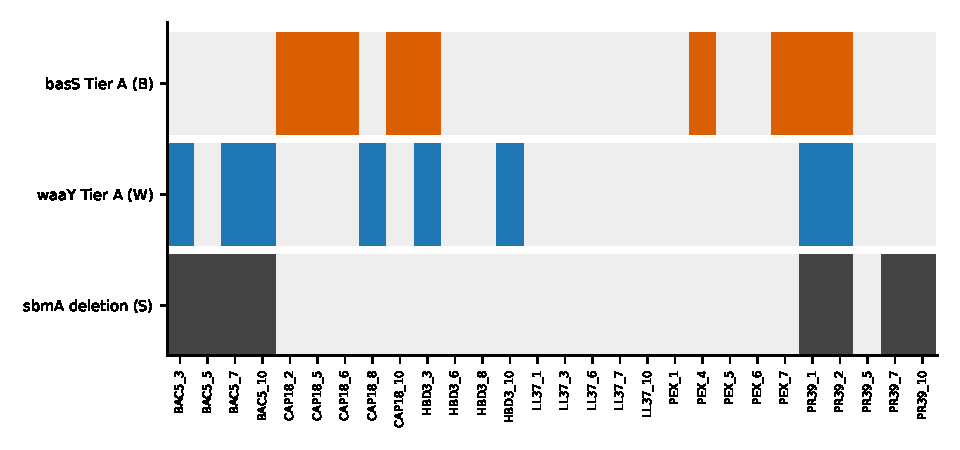
\includegraphics[width=0.95\textwidth]{fig_line_grid.pdf}\caption{Membership of the 28 sequenced adopted-AMP Spohn lines in the sbmA-deletion set (S), the waaY Tier A set (W) and the basS Tier A set (B). Data: \texttt{results/line\_dependence\_a10\_corrected\_universe28.json}.}\label{fig:grid}\end{figure}

\subsection{The basS and pmrB mapping (A11)}
E.\ coli BasS (P30844, 363 aa) and \textit{S.\ typhimurium} LT2 PmrB (P36557, 356 aa; UniProt names basS, parB, pmrB) share 306 identities (84.3\% of the longer sequence; length ratio 0.981), meeting the locked name-level rule (at least 70\% and ratio at least 0.9). A simple alignment (+1/$-1$/$-2$) was used because BLOSUM62 was unavailable; 84.3\% is far from the boundary. Sequence similarity supports orthology, not functional equivalence.

\subsection{Recurrence outside sbmA-deletion lines (A12, A14)}\label{sec:a12}
A12 excluded the eight sbmA-deletion lines and intergenic and Tier B events, leaving 20 lines (CAP18 5, PEX 5, LL-37 5, HBD3 4, PR39 1) and 64 mapped Tier A events. The statistic T counted (AMP, gene) pairs with Tier A hits in at least three same-AMP lines. Observed T was 4 (Table~\ref{tab:a12}). The null redrew each line's number of distinct genes from the 4{,}318 CDS in proportion to length (null mean $1.2\times10^{-4}$; 0 of 100{,}000 reps $\ge4$), so $p<10^{-5}$ under that null. The first run counted yejK and yejL (one intergenic event pair) in violation of the lock (T=6); it was corrected and both files are kept. A14 resolved the seven excluded events whose gene names are old synonyms (yejM$\to$lapC, yciM$\to$lapB, yebS$\to$letA, yebT$\to$letB, ybiH$\to$cecR; each a unique reviewed UniProt K-12 entry) and the verdict was unchanged (71 mapped events, T=4, $p<10^{-5}$).

\begin{table}[h]\centering\small\caption{Within-AMP Tier A recurrence outside sbmA-deletion lines (A12; A14 unchanged).}\label{tab:a12}
\begin{tabular}{llr}\toprule AMP & Gene & Lines hit\\\midrule CAP18 & basS & 4\\ LL-37 & lptC & 3\\ LL-37 & wzzE & 3\\ HBD3 & basR & 3\\\bottomrule\end{tabular}\end{table}

The null treats genes as independent draws weighted by length. It ignores insertion-sequence hotspots, linked or co-transcribed genes and mutation-rate heterogeneity, so the extreme tail value should not be read as a precise probability. basS and basR are one two-component system, and lptC and wzzE share the line LL37\_3. Lines within an AMP are not independent, and strata hold only four or five lines.

\subsection{A second organism, exploratory (A13, A13b)}
A13 applied the same statistic to the 16 Blanco evolved lines against 4{,}324 \textit{S.\ maltophilia} D457 CDS (NC\_017671.1). As locked, name-only mapping resolved only 5 of 16 events (RefSeq carries no sspB or mraW symbols), giving T=0 and $p=1.0$: \textbf{not testable as locked}, an annotation gap and not a finding. A13b added two mappings chosen after seeing which genes recurred (mraW$\to$rsmH; sspB$\to$the single CDS annotated ``ClpXP protease specificity-enhancing factor''). Then 14 of 16 events mapped, T=2 (PR-39: 6 of 8 lines; LL-37 rsmH: 3 of 8), and 0 of 100{,}000 reps reached 2 ($p<10^{-5}$). Because the mapping was chosen post hoc, this is \textbf{exploratory} and is not counted as a clean replication. It shows the phenomenon, not the same genes. Blanco lines come from a shared parent, which can inflate recurrence. Bac7 2023 (3 strains) was not testable.

\subsection{The 09d gate search (A15)}\label{sec:a15}
Before searching, criteria were locked: a PubMed-indexed paper independent of Spohn 2019 with a defined perturbation of basS, basR, lptC or wzzE (or the \textit{Salmonella} ortholog for basS) and a measured change in MIC or killing for the same AMP or family, with the direction stated. Five PubMed queries returned 20 distinct PMIDs, screened by abstract, with one full text read. The results:
\begin{itemize}\setlength\itemsep{1pt}
\item \textbf{basS/pmrB: partial.} Lofton et al.\ 2013 (PMID 23894360) found pmrB mutations (H164R in an LL-37 isolate; R13H in a wheat-germ-histone isolate) in passaged \textit{Salmonella} lineages. The reconstituted R13H gave only a small resistance increase, to wheat germ histones; the authors report the assay was not sensitive enough to show an effect and that pmrB had negligible effect in combinations. An LL-37 effect of pmrB is therefore not demonstrated.
\item \textbf{waaY:} the same paper shows a reconstituted waaY deletion gives about 2 to 4 logs higher survival against all three peptides including LL-37. This is independent functional support on the \textit{Salmonella} side, but waaY is not among the surviving genes, and it does not rescue A9.
\item \textbf{basR/pmrA: partial.} PmrA-PmrB governs resistance to polymyxin and other cationic peptides in \textit{Salmonella} (PMIDs 8955307, 11035717), but one report states PmrA-PmrB was not responsible for NP-1 defensin sensitivity, and another finds peptide-specific pmrA effects (PMID 29267354). No hBD3 measurement was found.
\item \textbf{lptC:} no qualifying record. \textbf{wzzE:} no hit.
\end{itemize}
Mass spectrometry was not applicable because no peptide is named. The gate is \textbf{unmet}.

\section{Discussion}
The lane's original objective, predicting resistance emergence from sequence features, failed its locked tests on the available data, and the data structure explains why: the labels are few, nested and partly censored. The pivot to mutation recurrence has produced one reading that survives its own controls so far, namely that the same genes are hit repeatedly under the same AMP in independent lines beyond what a length-weighted null expects. Four pairs in 20 lines is a small base, and the null is simple; the finding is hypothesis-generating. The affected genes (a two-component system, an LPS transport protein and an O-antigen chain length regulator) are all outer-membrane or LPS related, which is plausible but is not tested here.

Three earlier readings should not be repeated. First, sbmA recurrence cannot be called convergent selection: it does not beat a mutation-opportunity null, and most of its block evidence is breakpoint driven by IS elements. Second, waaY is not shown to depend on the sbmA-deletion lines; the briefly reported $p=0.0046$ came from a wrong denominator. Third, waaY/phoP concordance with \textit{Salmonella} is not established. Independent evidence that pmrB, phoP and waaY mutations arise under LL-37 passaging in \textit{Salmonella} (Lofton et al.\ 2013) is partial corroboration of the idea that two-component and LPS-core genes are recurrent targets, but it comes from a study this lane had already mined (and rated partial in the A2 mining log) rather than an independent replication of the \textit{E.\ coli} lines.

\section{Limitations}
(i) The null model is length-weighted and ignores mutation hotspots and linkage. (ii) Spohn strata hold 4 to 5 lines per AMP, and lines within an AMP are not independent. (iii) A13b rests on a post hoc mapping, and Blanco lines share a parent. (iv) Several analyses were run after the analyst had seen related counts; each lock states that exposure. (v) Reference-genome features were used, not each line's own assembly. (vi) The PubMed search was bounded: abstracts of 20 records and one full text. (vii) Several first-run results were wrong and were corrected; the originals are kept in the repository.

\section{Claim state and closing condition}
\textbf{Survives, descriptively:} within-AMP Tier A recurrence beyond a length-weighted null in lines without sbmA deletion (Section~\ref{sec:a12}), with the second-organism observation (A13b) labelled exploratory and Lofton 2013 cited as independent but partial corroboration. \textbf{Does not survive:} the 09d gate, sbmA recurrence exceeding mutation opportunity, waaY concordance, and waaY dependence on sbmA-deletion lines. No candidate peptide is nominated and no discovery is claimed. The gate would close only with a targeted functional test, for example a basS, lptC or wzzE allele measured against LL-37 or CAP18 MIC or killing in \textit{E.\ coli} BW25113, with a prespecified direction; no such test has been run.

\section{Length of this document}\label{sec:length}
The body of this document (Sections 1 to 7, excluding the appendix, references and front matter) is about \textbf{6 pages} (it ends on page 7 of an 8-page PDF; page 8 holds the appendices). The repository requires a 50+ page paper; that requirement is \textbf{unmet}. The evidence committed so far supports about this much honest text, and the document has not been padded.

\clearpage\appendix
\section{Disclosed deviations}
\begin{table}[!h]\centering\small\caption{Deviations disclosed in the repository, with their handling.}\label{tab:dev}
\begin{tabular}{p{0.22\textwidth}p{0.42\textwidth}p{0.28\textwidth}}\toprule Analysis & Deviation & Handling\\\midrule
A1 & Assumed sequence-level benchmark not supported; AUROC dropped & Disclosed in A1.2\\
A7b & Blanco (\textit{S.\ maltophilia}) placed in the \textit{E.\ coli} universe & \textit{E.\ coli}-only sensitivity $p=0.116$ reported\\
A10 & Lock said 120 lines; first run used 60; correct universe is 28 & First run withdrawn and kept; corrected $p=0.601$\\
A11 & BLOSUM62 not available; empty first pin replaced & Simple alignment; margin large\\
A12 & First run omitted the intergenic exclusion (T=6) & Corrected (T=4); both files kept\\
A13 & Name-only mapping resolved 5 of 16 events & Reported not testable\\
A13b & Mapping chosen after seeing recurring genes & Labelled exploratory\\
A15 & Search limited to abstracts plus one full text & Stated in Section~\ref{sec:a15}\\\bottomrule\end{tabular}\end{table}

\section{Reproducibility}
Scripts are in \texttt{scripts/}; results in \texttt{results/}; locks and result documents in \texttt{docs/}. Lock commits: A7 \texttt{036e075}; A7b \texttt{9e50efd}; A8 \texttt{d60c916}; A9 \texttt{35256e1}; A10 \texttt{7d0699e}; A11 \texttt{458119f}; A12 \texttt{57e242c}; A13 \texttt{36fe1c2}; A13b \texttt{f27e8cf}; A14 \texttt{81ffe43}; A15 \texttt{9504af1}. Unit tests live in \texttt{tests/}. Primary sources: Spohn et al.\ 2019 (Supplementary Data 5); Blanco et al.\ 2020; Bac7 2023 (supplement); Lofton et al.\ 2013, PLoS One 8(7):e68875 (PMID 23894360); PMIDs cited in Section~\ref{sec:a15}.
\end{document}
